\section{Лекція 3: Рядки}
\subsection{Створення рядків в Python} 
\begin{frame}
% \frametitle{Створення рядків в Python}
% \insertsection
% \insertsubsection
Рядок - упорядкований набір символів. Рядок - незмінний тип даних.
\begin{itemize}
  \item В одинарних лапках 'Python'
  \item В подвійних лапках "Python"
  \item 
  В потрійних лапках '''Python
  
  is the best!'''
  \item Символ переноса рядка \textbackslash n
 \end{itemize}

\end{frame}

\begin{frame}
\frametitle{Операції над рядками}
\begin{itemize}
  \item Конкатенація рядків (оператор \texttt{+})
  \item Повторення рядків (оператор \texttt{*})
  \item Функція \texttt{str}
  \item Довжина рядка. Функція \texttt{len}
  \item Оператор входження \texttt{in}
 \end{itemize}

\end{frame}

\begin{frame}
\frametitle{Порівняння рядків}
\begin{itemize}
  \item Дорівнює \texttt{==} або не дорівнює \texttt{!=}
  \item Більше \texttt{>} або менше \texttt{<}
  \item Функція \texttt{ord}
\end{itemize}
\begin{figure}
\begin{center}
 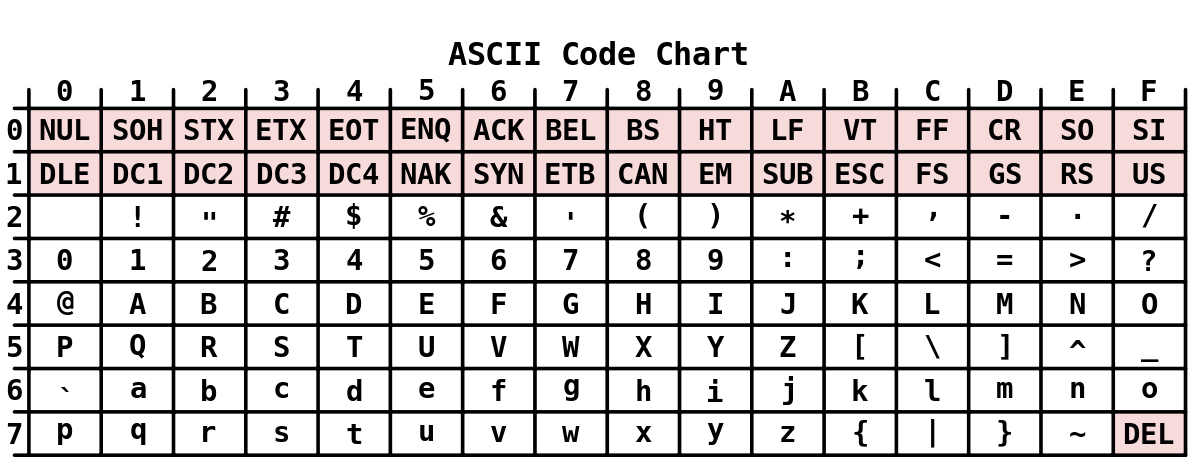
\includegraphics[width=0.8\textwidth]{pictures/ASCII-Table.png}
\caption{Таблиця ASCII}
\label{ASCII-Table} 
\end{center}
\end{figure}
\end{frame}

\begin{frame}
\frametitle{Елементи рядків}
Щоб отримати  i-й елемент рядка s використовується конструкція s[i]. Індекс i змінюється від 0 до len(s) - 1 (або від -1 до -len(s)).
\begin{figure}
\begin{center}
 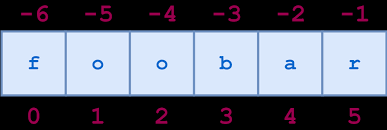
\includegraphics[width=0.5\textwidth]{pictures/string.png}
\caption{Елементи рядка}
\label{string} 
\end{center}
\end{figure}
\end{frame}

\begin{frame}
\frametitle{Зріз рядка}
Зріз (slice) — витяг із рядка одного символу або деякого фрагмента підрядка чи підпослідовності.

\begin{center}
\LARGE{s[start:stop:step]}
\end{center}
\end{frame}

\begin{frame}
\frametitle{Методи рядків}
\begin{center}
\texttt{об'єкт.метод(аргументи)}
\end{center}
\begin{figure}
\begin{center}
 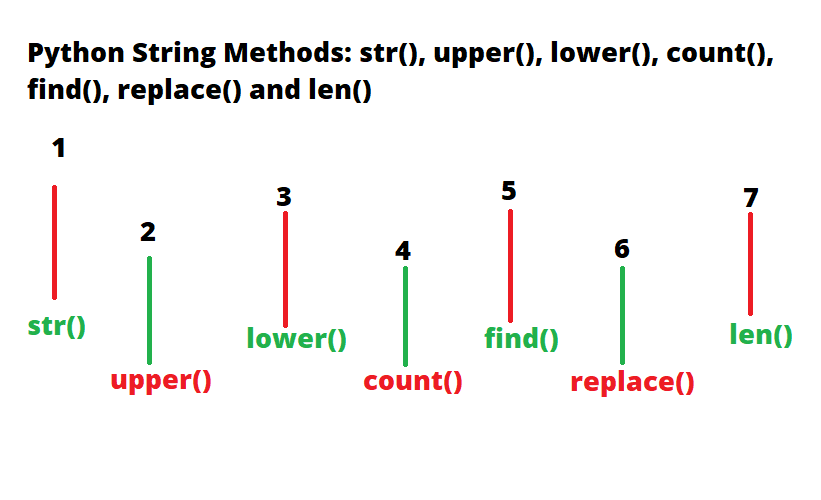
\includegraphics[width=0.5\textwidth]{pictures/python-string-methods.png}
\caption{Методи рядків}
\label{python-string-methods} 
\end{center}
\end{figure}
\end{frame}

\begin{frame}
\frametitle{Методи рядка s}
\begin{itemize}
  \item s.upper() - перетворює всі маленькі літери у великі;
  \item s.lower() - перетворює всі великі літери в маленькі;
  \item s.count(sub[, start[, end]]) - підрахунок кількості підрядків в рядку;
  \item s.find(sub[, start[, end]]) - індекс першого входження підрядка в рядку (find - пошук зліва направо, rfind - пошук зправа наліво);
  \item s.index(sub[, start[, end]]) - аналогічно до find, в разі не знаходження повертає помилку (find повертає -1);
\end{itemize}
\end{frame}

\begin{frame}
\frametitle{Методи рядка s}
\begin{itemize}
 \item s.replace(old, new[, count=-1]) - заміна підрядка old на підрядок new (count - кількість замін, count = -1 - без обмежень);
 \item s.isalpha() - повертає істину якщо рядок повністю складається із літер (інакше -повертає брехню);
 \item s.isdigit() - повертає істину якщо рядок повністю складається із цифр (інакше -повертає брехню);
 \item s.rjust(width[, fillcar=' ']) - повертає рядок заданої ширини width, fillcar - символи, що за потреби додаються зліва (у функції ljust - зправа);
\end{itemize}
\end{frame}

\begin{frame}
\frametitle{Методи рядка s}
\begin{itemize}
 \item s.split(sep=None, maxsplit=-1) - розбиває рядок за вказаним символом sep;
 \item s.join(list) - поєднує елементи списка list через роздільник s;
 \item s.strip(list) - видаляє всі символи пропусків та переносів рядків напочатку та вкінці рядка (rstrip - тільки зліва, lstrip - тільки зправа).
\end{itemize}
\end{frame}

\begin{frame}
\frametitle{Спеціальні символи рядків}
\tiny{
\begin{table}
  \caption{Спеціальні символи}
  \label{tab:}

  \begin{center}
    \begin{tabular}{|p{1.2cm}|p{3.5cm}|p{1.2cm}|p{3.5cm}|}
    \hline
     \textbf{Позначення}  & \textbf{Опис} & \textbf{Позначення}  & \textbf{Опис} \\
     \hline
      \textbackslash n & Перевод рядка & \textbackslash \textbackslash & Символо зворотнього слеша \\
     \hline
           \textbackslash ' & Символ апострофа & \textbackslash " & Символ подвійної лапки \\
     \hline
           \textbackslash a & Звуковий сигнал & \textbackslash b & Емуляція клавіші BackSpace \\
     \hline
           \textbackslash f & Переклад формату & \textbackslash r & Повернення каретки \\
     \hline
           \textbackslash t & Горизонтальна табуляція (4 пропуски) & \textbackslash v & Вертикальна табуляція \\
     \hline
           \textbackslash 0 & Симовол Null (не признак кінця рядка) & \textbackslash xhh & Символ з шістнадцятковим кодом hh \\
     \hline
           \textbackslash ooo & Символ з вісімковим кодом ooo  & \textbackslash N\{id\} & Ідентифікатор із кодової таблиці Unicode \\
     \hline
           \textbackslash uhhhh & 16-ти бітний символ Unicode в шістнадцятковій формі & \textbackslash Uhhhhhhhh &  32-х бітний символ Unicode в шістнадцятковій формі\\
     \hline
    \end{tabular}
  \end{center}
\end{table}
}
\end{frame}

\begin{frame}
\frametitle{"Сирі" (raw) рядки}
Якщо перед рядком поставити літеру \texttt{r}, то всі символи в ньому будуть сприйматися так, як вони написані.
\begin{figure}
\begin{center}
 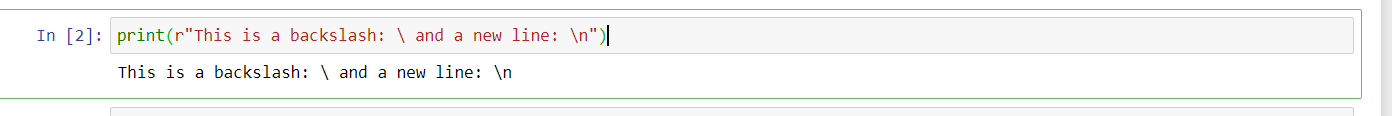
\includegraphics[width=\textwidth]{pictures/raw_string.png}
\caption{Приклад сирого рядка}
\label{raw_string} 
\end{center}
\end{figure}
\end{frame}

\begin{frame}
\frametitle{Методи формування рядків}
name = "Bruce"

age = 35
\begin{itemize}
  \item "My name is " + name + " and my age is " + str(age)
  \item "My name is \{0\} and my age is \{1\}".format(name, age)
  \item "My name is \{fio\} and my age is \{old\}".format(fio=name, old=age)
  \item f"My name is \{name\} and my age is \{age\}"
\end{itemize}
\end{frame}
